\documentclass[varwidth]{standalone}

\usepackage{tikz}
\usepackage{subcaption}
% \input{set-caption}

\tikzset{
	,thick
	,font = \ttfamily\bfseries\small
	,mynode/.style  = {circle, draw=black, align=center, fill=none}
	,mynoder/.style = {circle, draw=black, align=center, fill=red!40}
	,edgen/.style = {-}
	,edger/.style = {->, thick, blue}
}

% arara: pdflatex: { draft: yes }
% arara: pdflatex: { synctex: no }
% arara: latexmk: { clean: partial }
\begin{document}
% \begin{preview}
% \begin{minipage}{\linewidth}\centering
\begin{figure}
\begin{subfigure}[b]{.5\linewidth}\centering
	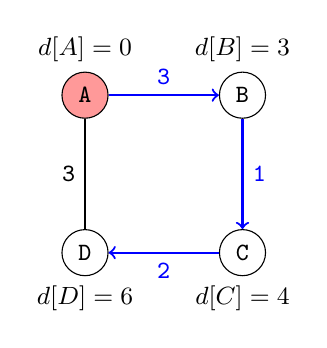
\begin{tikzpicture}
		\node[mynoder, label={above: \(d[A]=0\) }] at (0.0, 2.0) (a) {A};
		\node[mynode,  label={above: \(d[B]=3\) }] at (2.0, 2.0) (b) {B};
		\node[mynode,  label={below: \(d[C]=4\) }] at (2.0, 0.0) (c) {C};
		\node[mynode,  label={below: \(d[D]=6\) }] at (0.0, 0.0) (d) {D};
		\draw[edger] (a) edge node[above] {3} (b);
		\draw[edger] (b) edge node[right] {1} (c);
		\draw[edger] (c) edge node[below] {2} (d);
		\draw[edgen] (d) edge node[left]  {3} (a);
	\end{tikzpicture}
	\caption{Soluzione ammissibile}%
	\label{fig:etichetta}
\end{subfigure}
\begin{subfigure}[b]{.5\linewidth}\centering
	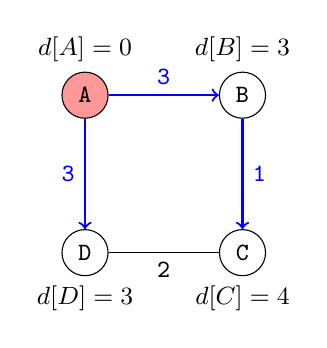
\begin{tikzpicture}
		\node[mynoder, label={above: \(d[A]=0\) }] at (0.0, 2.0) (a) {A};
		\node[mynode,  label={above: \(d[B]=3\) }] at (2.0, 2.0) (b) {B};
		\node[mynode,  label={below: \(d[C]=4\) }] at (2.0, 0.0) (c) {C};
		\node[mynode,  label={below: \(d[D]=3\) }] at (0.0, 0.0) (d) {D};
		\draw[edger] (a) edge node[above] {3} (b);
		\draw[edger] (b) edge node[right] {1} (c);
		\draw[edgen] (c) edge node[below] {2} (d);
		\draw[edger] (a) edge node[left] {3} (d);
	\end{tikzpicture}
	\caption{Soluzione ottima}%
	\label{fig:etichetta}
\end{subfigure}
\caption{Alberi di cammini minimi}
\end{figure}
% \end{minipage}
% \end{preview}
\end{document}
